\documentclass[11pt,a4paper]{article}

\usepackage[utf8]{inputenc}
\usepackage[T1]{fontenc}
\usepackage[english]{babel}
\usepackage{geometry}
\usepackage{graphicx}
\usepackage{booktabs}
\usepackage{tabularx}
\usepackage{array}
\usepackage{float}
\usepackage{hyperref}
\usepackage{xcolor}
\usepackage{tikz}
\usepackage{enumitem}
\usepackage{caption}

\geometry{margin=2.3cm}
\graphicspath{{../results/plots/}{results/plots/}}
\hypersetup{
  colorlinks=true,
  linkcolor=black,
  citecolor=black,
  urlcolor=blue
}
\setlist[itemize]{topsep=2pt,itemsep=2pt,parsep=0pt}
\setlist[enumerate]{topsep=2pt,itemsep=2pt,parsep=0pt}
\emergencystretch=3em

\title{\textbf{Movie Search on Spin/WASM and OCI}\\
\large Comparing WebAssembly as isolation for microservices}
\author{LSC Project}
\date{24 May 2026}

\begin{document}
\maketitle

\begin{abstract}
This project compares the same HTTP application running under two isolation models:
Spin/wasmtime as a WASI component and a native Rust server packaged as an OCI image.
After an initial analysis, we abandoned comparing Spin with full Meilisearch, because
official Meilisearch relies on LMDB and assumptions typical of native runtimes that could
not be ported 1:1 to WASI within the project timeline. Instead, we built a custom,
deterministic \texttt{movie-search} service in which Spin and OCI share the same application
code, fixture, and API semantics. Results show full functional parity, a shorter first
search request on Spin, very fast OCI responses for a simple empty query, and a clearly
larger observed Spin process RSS under load. We conclude that Spin/WASM is a reasonable
candidate for isolated, short-lived HTTP microservices, but OCI containers remain a more
mature and predictable operational choice, especially for storage-heavy services.
\end{abstract}

\section{Goal and context}

The project examined whether WebAssembly run via Spin and wasmtime can serve as a practical
isolation substrate for serverless-style microservices compared with a classic OCI container.
WebAssembly is a binary instruction format designed as a portable compilation target for
programming languages, including outside the browser \cite{webassembly}. WASI extends this
model with system interfaces such as files, networking, clocks, and randomness while keeping
a controlled permission model \cite{wasmtime-intro,wasi-interfaces}. Spin is a framework for
building WebAssembly microservices and applications, with a simple \texttt{spin build} and
\texttt{spin up} workflow, HTTP triggers, and WASI-compatible languages \cite{spin}. Wasmtime
acts as the runtime for WebAssembly, WASI, and the Component Model in this stack
\cite{wasmtime-intro}.

The reference point is OCI: an open standard for describing and running container images,
built around runtime, image, and distribution specifications \cite{oci}. A Docker container
packages an application and its dependencies into a standardized unit that is isolated from
the host and portable across environments \cite{docker-container}. The research question is
therefore: what do we get when we run the same application code once as a WASI component and
once as a native process in a container?

\section{Pivot away from Meilisearch}

The first direction assumed comparing Meilisearch in a container with a Spin-hosted variant.
A feasibility analysis showed that this would be technically unfair. Official Meilisearch
stores data in \texttt{data.ms} and uses LMDB as its storage engine; LMDB relies on
memory-mapped files \cite{meilisearch-storage}. Meilisearch backups distinguish snapshots,
i.e.\ a copy of the \texttt{data.ms} database, from dumps portable across Meilisearch versions
\cite{meilisearch-backup}. That remains Meilisearch's data model, not a portable index for a
custom WASI component.

In addition, local attempts to compile upstream Meilisearch layers to \texttt{wasm32-wasip2}
stopped on dependencies such as \texttt{ring}, Tokio, and expected storage blockers related
to LMDB and mmap. The project therefore shifted from ``port Meilisearch'' to ``compare the
same custom microservice under two runtime isolations.'' The benchmark thus measures
deployment and isolation differences, not search-engine semantics.

\section{Application and architecture}

The final application is \texttt{movie-search}: a simple HTTP service written in Rust. Both
runtimes use the same \texttt{movie-search-core} library, the same \texttt{fixtures/movies.json}
file, and the same ranking rules. The fixture contains 44\,471 unique movies after deduplication
by \texttt{id}. Search is deterministic: tokenization on non-alphanumeric characters,
case-insensitive substring matching, sorting by the number of matched tokens, field weights
\texttt{title > genre > overview}, and finally ascending \texttt{id}. Typo tolerance, synonyms,
and Meilisearch-specific rules were intentionally not implemented.

\begin{figure}[H]
\centering
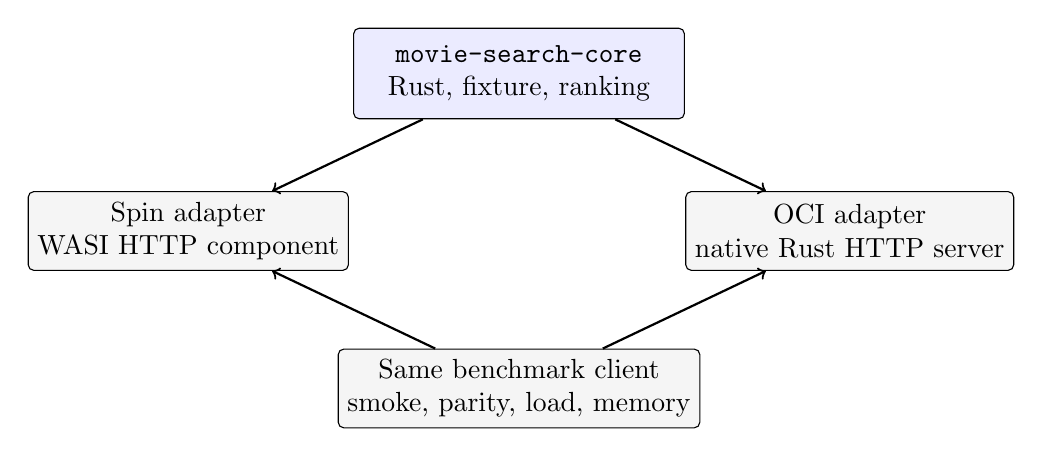
\begin{tikzpicture}[
  box/.style={draw, rounded corners=2pt, minimum width=3.4cm, minimum height=1.0cm, align=center, fill=gray!8},
  core/.style={draw, rounded corners=2pt, minimum width=4.2cm, minimum height=1.15cm, align=center, fill=blue!8},
  arrow/.style={->, thick}
]
\node[core] (core) at (0,0) {\texttt{movie-search-core}\\Rust, fixture, ranking};
\node[box] (spin) at (-4.2,-2) {Spin adapter\\WASI HTTP component};
\node[box] (oci) at (4.2,-2) {OCI adapter\\native Rust HTTP server};
\node[box] (client) at (0,-4) {Same benchmark client\\smoke, parity, load, memory};
\draw[arrow] (core) -- (spin);
\draw[arrow] (core) -- (oci);
\draw[arrow] (client) -- (spin);
\draw[arrow] (client) -- (oci);
\end{tikzpicture}
\caption{Final architecture: one application core, two runtime adapters.}
\end{figure}

The public API is shared by both variants: \texttt{GET /health}, \texttt{GET /version},
\texttt{GET /stats}, \texttt{GET /movies?offset=\&limit=}, and \texttt{POST /search}. Spin
runs locally on port 8080, and the OCI variant on port 8081.

\section{Methodology}

Before performance measurement, we run unit tests, build the Spin component, build the OCI
image, and run smoke/parity checks. The script \texttt{benchmarks/compare\_results.sh} compares
engine, document count, hit count, and \texttt{hit.id} lists for queries \texttt{space},
\texttt{toy story}, \texttt{dark knight}, \texttt{romance}, and the empty query.

The full benchmark was run with \texttt{benchmarks/run\_all.sh}. It includes 20 cold-start
repetitions, load tests on \texttt{POST /search} for queries \texttt{space} and empty at
concurrency 10, 50, 100, and 200, and memory samples in idle and under-load states.
Environment: Apple M4, 10 cores, 24 GiB RAM, macOS 15.6, Spin 3.6.3, Docker 28.5.1, Rust
1.95.0. The Docker image was built before the cold-start measurement; build time is not part
of the result.

An important limitation concerns memory. OCI is measured via \texttt{docker stats} and reflects
the container's perspective. Spin is measured as host process-tree RSS. These numbers are useful
for comparing observed overhead but are not an identical memory accounting layer.

\section{Results}

All functional and load tests completed without response validation errors. The parity check
confirmed identical functional results for both runtimes.

\begin{table}[H]
\centering
\caption{Cold start: 20 repetitions per system.}
\begin{tabular}{llrrrr}
\toprule
System & Metric & Median [ms] & p95 [ms] & p99 [ms] & Errors \\
\midrule
OCI & \texttt{/health} & 20.982 & 28.420 & 36.325 & 0 \\
OCI & \texttt{/health + /search} & 307.755 & 376.983 & 446.288 & 0 \\
Spin & \texttt{/health} & 141.357 & 144.220 & 152.354 & 0 \\
Spin & \texttt{/health + /search} & 205.649 & 217.504 & 218.947 & 0 \\
\bottomrule
\end{tabular}
\end{table}

\begin{figure}[H]
\centering
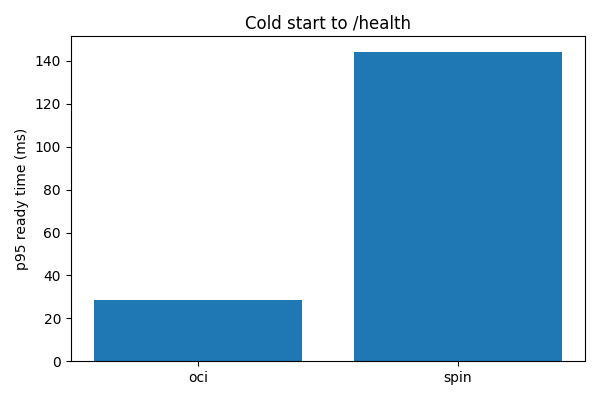
\includegraphics[width=0.62\linewidth]{cold_start_p95.png}
\caption{p95 cold start until the first successful \texttt{/health}.}
\end{figure}

In this environment, the container reached \texttt{/health} readiness faster, while Spin
completed the cold start plus first search sequence faster. This should be interpreted as a
property of the specific implementation and measurement approach: \texttt{/health} is a cheap
readiness endpoint, whereas \texttt{/search} exercises the application's real work path.

\begin{table}[H]
\centering
\caption{Load test: request rate and p95 latency.}
\resizebox{\linewidth}{!}{
\begin{tabular}{llrrrrrrrr}
\toprule
System & Query & \multicolumn{2}{c}{c=10} & \multicolumn{2}{c}{c=50} &
\multicolumn{2}{c}{c=100} & \multicolumn{2}{c}{c=200} \\
 & & req/s & p95 ms & req/s & p95 ms & req/s & p95 ms & req/s & p95 ms \\
\midrule
OCI & empty & 3314.9 & 5.4 & 2931.1 & 26.8 & 2934.6 & 52.3 & 2899.0 & 95.7 \\
Spin & empty & 132.8 & 100.0 & 129.1 & 643.5 & 123.0 & 1516.1 & 123.3 & 3636.0 \\
OCI & space & 54.0 & 210.8 & 46.2 & 2164.9 & 58.0 & 1899.6 & 61.5 & 3747.5 \\
Spin & space & 77.2 & 168.3 & 70.3 & 1264.6 & 74.5 & 2491.2 & 78.3 & 6073.3 \\
\bottomrule
\end{tabular}
}
\end{table}

\begin{figure}[H]
\centering
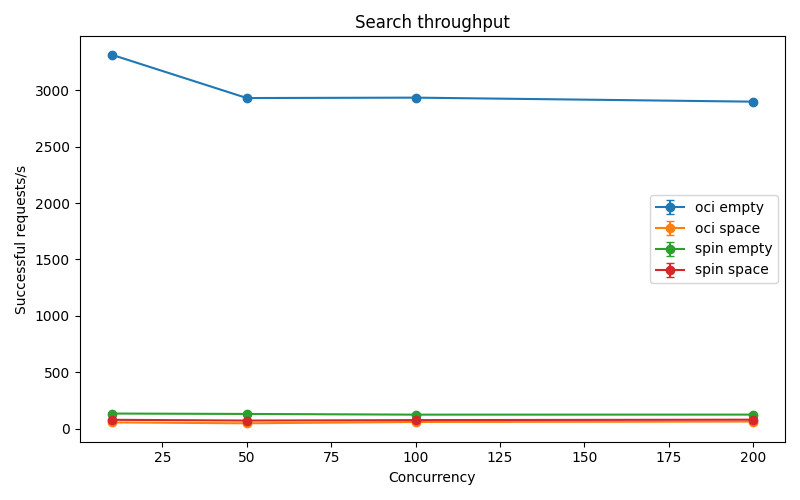
\includegraphics[width=0.49\linewidth]{load_throughput.png}
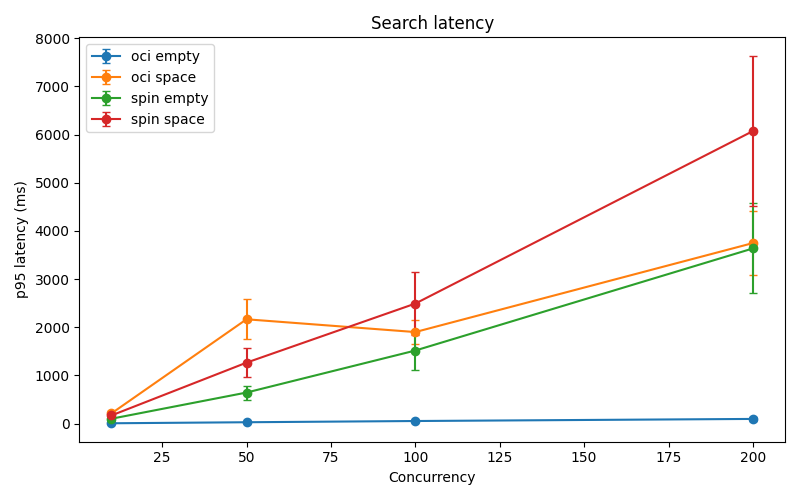
\includegraphics[width=0.49\linewidth]{load_latency_p95.png}
\caption{Throughput and p95 latency for \texttt{POST /search}.}
\end{figure}

For the empty query, the native OCI server was decisively faster. This is a low application-cost
path: it returns the first documents deterministically without expensive text filtering. For the
\texttt{space} query, the picture is more nuanced. Spin achieved higher throughput but worse
latency tails at very high concurrency. This suggests the benchmark measures not only isolation
but also the interaction of simple linear scanning over 44\,471 records with each runtime's HTTP
model and scheduling.

\begin{table}[H]
\centering
\caption{Memory: maximum of observed samples.}
\begin{tabular}{llrr}
\toprule
System & Phase & Source & Max [MiB] \\
\midrule
OCI & idle & \texttt{docker stats} & 29.8 \\
OCI & load & \texttt{docker stats} & 31.9 \\
Spin & idle & host process RSS & 104.8 \\
Spin & load & host process RSS & 493.5 \\
\bottomrule
\end{tabular}
\end{table}

\begin{figure}[H]
\centering
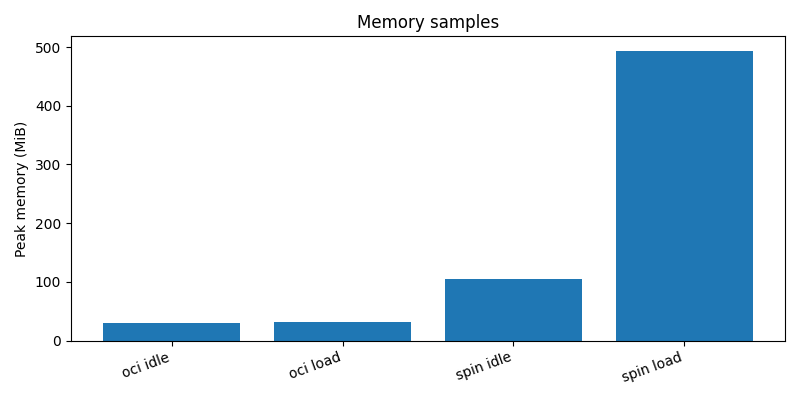
\includegraphics[width=0.68\linewidth]{memory_peak.png}
\caption{Peak memory samples for idle and load.}
\end{figure}

Memory is the strongest argument against the simple claim that the WASM variant is always
lighter. In this project, the observed Spin process together with wasmtime had higher RSS than
the OCI container. At the same time, this is not a full production cost model, because Docker
reports memory from the container perspective while Spin is measured from the host process
perspective. The final report therefore draws a cautious conclusion: Spin offers an interesting
capability-oriented isolation model, but it requires deliberate measurement and does not
automatically guarantee lower overhead.

\section{Demo}

The presentation demo does not run the full benchmark live. Measurements are collected
beforehand; during the presentation we show a reproducible path:

\begin{enumerate}
  \item start Spin on \texttt{127.0.0.1:8080} and OCI on \texttt{127.0.0.1:8081};
  \item check \texttt{/health}, \texttt{/version}, and \texttt{/stats};
  \item run one \texttt{space} search;
  \item run \texttt{benchmarks/compare\_results.sh};
  \item show the final charts and CSV files.
\end{enumerate}

If the live environment fails, the fallback plan is to show saved artifacts:
\path{results/raw}, \path{results/processed}, and \path{results/plots}. The full scenario is
in \path{demo/demo-script.md}.

\section{Reproducibility and limitations}

The repository is set up so results can be reproduced in a single run:

\begin{verbatim}
benchmarks/run_all.sh
\end{verbatim}

The script builds both variants, runs correctness tests, performs smoke/parity checks, collects
three kinds of raw CSV data, and generates processed files:
\path{results/processed/cold_start_summary.csv},
\path{results/processed/load_summary.csv}, and
\path{results/processed/memory_summary.csv}. Charts in this report come from
\path{results/plots}. Raw data from the final run are kept in \path{results/raw}; earlier pilot
data are not mixed with the final results.

There are three main interpretive limitations. First, the application does not use an inverted
index: \texttt{space} search is intentionally simple text scanning, so it does not compare
production search-engine quality. Second, cold-start measurement depends on the local host,
system cache, and the fact that the OCI image was built beforehand. Third, Spin and OCI memory
are measured from different tooling perspectives. Conclusions should therefore be treated as
the outcome of a controlled local experiment, not a universal characterization of all WASM and
container workloads.

\section{Conclusions}

The most important project outcome is methodological: the comparison is fair because both
runtimes execute the same application code and return identical results. Spin/WASM fits small,
isolated HTTP components, plugins, edge functions, and serverless workloads where portability,
sandboxing, and a simple capability-oriented model matter. OCI containers remain more mature
operationally: they have widespread tooling, stable resource accounting, a familiar deployment
model, and very good performance for simple native paths.

In our benchmark, OCI had faster \texttt{/health} readiness, Spin had a faster first search
request after startup, and load results depended strongly on the query. The empty query clearly
favored OCI, while the \texttt{space} query showed higher Spin throughput with worse latency tails
at high concurrency. The Meilisearch attempt remains a valuable appendix: a storage-heavy system
built on LMDB and mmap is not a good candidate for a simple WASI port without substantial
architectural changes.

\begin{thebibliography}{9}
\bibitem{webassembly}
WebAssembly, \textit{Official website}. \url{https://webassembly.org/}.

\bibitem{wasi-interfaces}
WASI.dev, \textit{Interfaces}. \url{https://wasi.dev/interfaces}.

\bibitem{wasmtime-intro}
Bytecode Alliance, \textit{Wasmtime Introduction}. \url{https://docs.wasmtime.dev/introduction.html}.

\bibitem{spin}
Fermyon, \textit{Develop serverless WebAssembly apps with Spin}. \url{https://www.fermyon.com/spin}.

\bibitem{oci}
Open Container Initiative, \textit{Open Container Initiative}. \url{https://opencontainers.org/}.

\bibitem{docker-container}
Docker, \textit{What is a Container?}. \url{https://www.docker.com/resources/what-container/}.

\bibitem{meilisearch-storage}
Meilisearch, \textit{Storage}. \url{https://www.meilisearch.com/docs/resources/internals/storage}.

\bibitem{meilisearch-backup}
Meilisearch, \textit{Backing up Meilisearch data}. \url{https://www.meilisearch.com/docs/resources/self_hosting/data_backup/overview}.
\end{thebibliography}

\end{document}
